documentclass(tikz)
\begin{document}
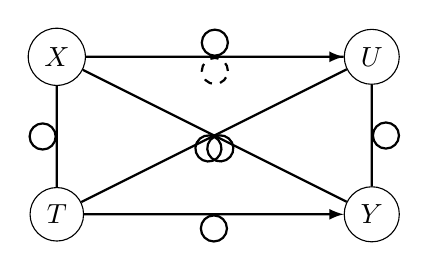
\begin{tikzpicture}[%
    every node/.style={draw,circle},
    >=latex,
    ]
    \node (x) at (-2, 0) {$X$};
    \node (u) at (2, 0) {$U$};
    \node (y) at (2, -2) {$Y$};
    \node (t) at (-2,-2) {$T$};
    \draw[->, thick]
        (x) -- node[sloped,below] {} (t)
        (u) -- node[sloped,below] {} (t)
        (u) -- node[sloped,above] {} (x)
        (u) -- node[sloped,above] {} (y)
        (x) -- node[sloped,below] {} (y)
        (t) -- node[sloped,below] {} (y);
    \draw[->, dashed, thick]
        (x) -- node[sloped,below] {} (u);
\end{tikzpicture}
\end{document}